

\documentclass{article}
\usepackage[utf8]{inputenc}
 \usepackage{hyperref}
 \usepackage{multirow}
 \usepackage[margin=1in]{geometry}
 \usepackage{enumitem}
\usepackage{graphicx}
\usepackage{xr}
\usepackage[T1]{fontenc}
\usepackage{lmodern}
\newcommand*{\escape}[1]{\texttt{\textbackslash#1}}
\newcommand*{\escapeI}[1]{\texttt{\expandafter\string\csname #1\endcsname}}
\newcommand*{\escapeII}[1]{\texttt{\char`\\#1}}

%\hypersetup{
%    colorlinks,
%    citecolor=black,
%    filecolor=black,
%    linkcolor=black,
%    urlcolor=black
%}

\usepackage{xcolor}
\usepackage{listings}
\lstset{basicstyle=\ttfamily,
  showstringspaces=false,
  commentstyle=\color{red},
  keywordstyle=\color{blue},
  backgroundcolor=\color{black!5} % set backgroundcolor
}



\title{\textit{MCXplore}: An Automated Framework for Validating Memory Controller
Designs}
\author{Mohamed Hassan and Hiren Patel}
\date{version1.0}
 
\begin{document}
 
\maketitle
 
\tableofcontents
 
\externaldocument{configuration_tbl}
\externaldocument{flow}
\externaldocument{TL}
\section{Introduction}
\textit{MCXplore} is an automation tool that generates tests to validate the memory system and evaluate its performance. 
The novel observation behind \textit{MCXplore} is the following. 
Regardless of various policies proposed for the memory system, the test pattern is still the same. 
This test pattern consists of a sequence of memory requests. 
Each request has three major components: the address, the transaction type (whether read or write), and the transaction size (the number of bytes to transfer). 
Based on this observation, instead of building a validation framework per memory policy, \textit{MCXplore} relies in the input test pattern to validate any memory policy. 
\textit{MCXplore} has two modes of operation: non model checking mode and model-checking mode.
\subsection{Non model checking mode}
In the first one, the user configures a set of parameters to generate the test that has the desired properties. 
These parameters represent the pattern required for the address and type of transactions in the test. 
This mode is suitable for validating common memory controller aspects such as:
\begin{enumerate}
\item Common page policies such as close-, open- and adaptive-page policies. 

\item Common address mapping schemes such as traditional address mappings with any segment order. For example, CH:RW:RNK:BNK:CL, CH:RW:BNK,RNK,CL, ..., etc. 
It is also suitable for non traditional mappings such as XOR address mapping, where bank bits are XORed with low-significant row bits. 

\end{enumerate}  

This mode has a set of predefined-- yet expandable-- patterns for each of the address segments as well as the transaction type. 
We tabulate currently implemented patterns in Table~\ref{tb:config_noMChk}. 
Although this model is easy to use, it does not necessarily cover the whole state space of the test pattern. 
%Consequently, we propose the second mode. 

To use this mode, the user does not need to specify any model to the tool as this mode is the default for \textit{MCXplore}. 
Alternatively, the user can specify this mode by setting the -m flag to \textbf{noMChk}. 
As the flow diagram in Figure~\ref{fig:flow} illustrates, the main script for this mode is \textit{\textbf{MCXplore\_noMChk.pl}}.



\subsection{Model Checking mode}
The second mode leverages model checking capabilities to cover the state space of the memory input test. 
Model checking automates the state-space exploration of the test generation,
and provides a formal methodology to define test properties.
We create two abstract models to express the stimulus test of the MC: a request interrelation model, \textbf{REQmdl}, and a command interaction model, \textbf{CMDmdl}, and we encode them as FSMs in the NuSMV model checker. The two NuSMV models are in \textbf{\textit{CMDmdl.smv}} and \textbf{\textit{REQmdl.smv}} under the \textbf{\textit{\textbackslash Models}} directory, respectively. 
the user is able to encode test properties as specifications expressed in temporal logic formulas. 
Formulas are negated such that they are true if required test properties do not exist. 
For examples of these formulas, see Section~\ref{sec:TL}.
As the flow diagram in Figure~\ref{fig:flow} illustrates, the main two script for these  two models are \textit{\textbf{MCXplore\_REQmdl.sh}} and \textit{\textbf{MCXplore\_CMDmdl.sh}}, respectively.

\section{Installation}

\subsection{Download} 

\begin{itemize}
\item

\textit{MCXplore} can be downloaded from here:

\url{https://caesr.uwaterloo.ca/mcxplore/},

 or directly from the git repository at:


\url{https://git.uwaterloo.ca/caesr-pub/mcxplore} 

\item 

You need also to download the NuSMV model checker tool from: 
\url{http://nusmv.fbk.eu/} and extract to /NuSMV directory
\end{itemize}
\subsection{Required tools}
\textit{MCXplore} is a combination of Shell and Perl scripts. 
Therefore, to properly use \textit{MCxplore}, please make sure that the following tools are installed in your system:
\begin{itemize}
\item Perl
\end{itemize} 

In addition, please make sure that you use the bash Unix shell. 



\begin{itemize}
\item For Linux and Mac OS users, simply switch to bash by running the following command:

\begin{lstlisting}[language=bash]
/bin/bash
\end{lstlisting}

or:

\begin{lstlisting}[language=bash]
chsh -s /bin/bash
\end{lstlisting}

\item For Windows users, there exist many tools to run bash scripts on Windows. 
Examples include: 

\begin{itemize}
\item Cygwin, \url{https://www.cygwin.com/}

\item win-bash, \url{http://win-bash.sourceforge.net/}
\end{itemize}

\end{itemize} 




 
\section{Usage}

%run [-m model |[-h]
%	echo "-m, --model		specify which model to use: \"CMDmdl\" for Model Checking Command model, \"REqmdl\" for Model Checking request model, or \"noMChk\" for the no model checking usage. noMChk is the default"
%	echo "-o, --out		  specify the output file name of the generated test. results/[model]/Test.trc is the default"
%	echo "-h, --help		prints out this usage message"          
The usage of \textit{MCXplore} is as simple as invoking the \textit{\textbf{MCXplore.sh}} script as follows:
\begin{lstlisting}[language=bash]
./ mcxplore [[-m model] [-o output_file] [-t DRAM_timing_file] [-s LTL_specs_file] |[-h]]

\end{lstlisting}
Table~\ref{tb:usage} illustrates the possible options and their description.
\begin{table}[h] 
\scriptsize
\centering
\caption{Usage arguments.\label{tb:usage}}
\begin{tabular}{|l|l|l|p{5cm}|p{5cm}|}
  \hline
   Short flag &  Long flag & \multicolumn{2}{l|}{Options} & Description\\
   \hline
  \multirow{3}{*}{-m} & \multirow{3}{*}{-{}-model} & CMDmdl & Model Checking Command model &   \multirow{3}{*}{Specify which model to use}\\ 
  
  & & REQmdl & Model Checking request model &\\
  & &noMChk& no model checking usage. noMChk is the default&\\
      
\hline


-o & -{}-out& \multicolumn{2}{l|}{Any valid file name}&specify the output file name of the generated test. results/[model]/Test.trc is the default\\

\hline


-t &  -{}-DDrTiming & \multicolumn{2}{l|}{Any valid file name} & specify the input timing file with DDR constraints. DDrTimings/DDR3\_1600.tim is the default\\

\hline

-s &  -{}-Spec &  \multicolumn{2}{l|}{Any valid file name} &	specify the input LTL specification file that models the test plan. LTLspec/CMDmdl.spec is the default\\

\hline

-h & -{}-help & \multicolumn{2}{l|}{No options}&prints out this usage message\\

\hline
\end{tabular}
\label{tb:vars}
\end{table}

 
\section{Configurations}

There are four categories of configuration parameters. 
the user can configure any of these parameters by modifying the \textbf{\textit{configuration.data}} file. 

\begin{enumerate}
\item Parameters that configure the syntax of the output test. 
Table~\ref{tb:syntax} tabulates these parameters with their explanation and options. 
The user can modify these parameters or add a different syntax by expanding the \textit{\textbf{GenerateTest.pl}} file. 
\begin{table*}[ht] 
\scriptsize
\centering
\caption{Test syntax parameters.\label{tb:syntax}}
\begin{tabular}{|l|p{0.5cm}|p{7cm}|p{5cm}|}
  \hline
   Parameter & \multicolumn{2}{l|}{Possible Values} & Description \\
  \hline
address\_length & \multicolumn{2}{l|}{Either $32$bits or $64$bits} & Number of address bits\\
\hline

initial\_address & \multicolumn{2}{l|}{Hex number aligns with the address\_length parameter} & Address of the first request in the test (default is 00000000 for $32$bit address)\\
\hline

initial\_type & \multicolumn{2}{l|}{Either "read" or "write"} & type the first request in the test\\
\hline


\multirow{4}{*}{syntax} & $11$ & Address\escape{t}Transaction\_size\escape{t}Type (tab separated). Example: 0x00003F87	64	R & \multirow{4}{*}{syntax of the output test} \\

&$12$ & Address\escape{t}Type (tab separated). Example: 0x00003F8		R&\\
&$21$ & Address\escape{s}Transaction\_size\escape{s}Type (space separated). Example: 0x00003F87 64 R&\\
&$22$ & Address\escape{s}Type (space separated). Example: 0x00003F87 R&\\
\hline

\multirow{3}{*}{type\_syntax} & $31$ & READ (or WRITE) & \multirow{3}{*}{syntax of the output type} \\

&$32$ & R (or W)&\\
&$33$ & Read (or Write)&\\

\hline
\end{tabular}
\label{tb:vars}
\end{table*}
\item Parameters that configure test semantics but are model-independent. 
This category includes two parameters: the number of requests in the test and the transaction size as Table~\ref{tb:config_noMChk} explains.
\begin{table*}[ht] 
\scriptsize
\centering
\caption{Model-independent configuration parameters.\label{tb:config}}
\begin{tabular}{|l|p{1.2cm}|p{9cm}|p{5cm}|}
  \hline
  Parameter & \multicolumn{2}{l|}{Possible Values} & Description \\
  \hline
number\_of\_requests &  \multicolumn{2}{l|}{Any positive integer} & total number of requests in the test\\ 
\hline
\multirow{2}{*}{transaction\_size} & \multicolumn{2}{l|}{Any positive integer} & {Number of bytes transferred per memory transaction} \\
& \multicolumn{2}{l|}{For instance, if it is a cache line size, it is 64B or 128B} &\\
\hline
\end{tabular}
\label{tb:vars}
\end{table*}

\begin{table*}[ht] 
\scriptsize
\centering
\caption{Test configuration parameters for noMChk mode.\label{tb:config_noMChk}}
\begin{tabular}{|l|p{1.2cm}|p{7cm}|p{4cm}|}
  \hline
  Parameter & \multicolumn{2}{l|}{Possible Values} & Description \\
  \hline
\multirow{5}{*}{transaction\_pattern} &  rd& All requests are read & \multirow{5}{*}{Pattern of request type}\\

&wr& All requests are write&\\
&sw& The test alternates between reads and writes (rd wr rd wr ....)&\\

&sw\%& User configures the percentage of switching by another parameter(switch)&\\
&random& The type of each request is randomly selected&\\
\hline
switch & \multicolumn{2}{l|}{An integer between $0$ and $100$} & The switching \%  between reads and writes in the test\\
%address\_pattern & X
\hline
 \multirow{6}{*}{row\_pattern} &hit& All requests target the same row& \multirow{6}{*}{The row (page) pattern of the test}\\
 &conflict& Each two consecutive requests target different rows&\\
 &random& Row bits of the request is chosen randomly&\\
 &custom\_hit& User configures the number of row hits by another parameter(num\_hits) &\\
 &linear& Each request target row $rw+1$, where $rw$ is the row of the precedent request&\\
 &locality\%&User configures the percentage of row locality by another parameter(locality)&\\
 \hline
 num\_hits & \multicolumn{2}{l|}{any non-negative integer such that num\_hits $<$ number\_of\_requests} & The number of row hits in the test  \\
 \hline
 locality & \multicolumn{2}{l|}{An integer between $0$ and $100$} &  The row locality \% in the test\\
 
 \hline
 
 \multirow{5}{*}{rank\_pattern} & same & all requests target same rank & The rank pattern of the test\\
 
 &interleave&Each two consecutive requests target different ranks&\\
 &random&Rank bits of the request is chosen randomly&\\
 &interleave\%&User configures the percentage of rank interleaving by another parameter(RankInterleave)&\\
 &linear&Each request target rank $rnk+1$, where $rnk$ is the rank of the precedent request&\\
 
 \hline
 RankInterleave & \multicolumn{2}{l|}{An integer between $0$ and $100$} & The rank interleaving \%  in the test\\
 
 \hline
 
bank\_pattern &  \multicolumn{2}{l|}{Same as rank\_inteleave values} & The bank pattern of the test\\

 \hline
 BankInterleave & \multicolumn{2}{l|}{An integer between $0$ and $100$} & The bank interleaving \%  in the test\\
  \hline
 
channel\_pattern &  \multicolumn{2}{l|}{Same as rank\_inteleave values} & The channel pattern of the test\\

 \hline
 ChannelInterleave & \multicolumn{2}{l|}{An integer between $0$ and $100$} & The channel interleaving \% in the test\\
 
%channel\_pattern & X
%column\_pattern & interleave
%
%BankInterleave & 50

%ChannelInterleave & 50
  \hline
\end{tabular}
\label{tb:vars}
\end{table*}
\item Pattern configuration parameters for the no model checking mode. 
Table~\ref{tb:config} illustrates these parameters, their possible values and their description. 

\item Address mapping parameters, which decides the bits assigned to each address segment (Channel, rank, bank, row and column). 
\begin{table*}[ht] 
\scriptsize
\centering
\caption{Address mapping parameters.}
\begin{tabular}{|l|p{9cm}|p{5cm}|}
  \hline
   Parameter & Description & Example\\
   
   row\_mask & Mask determines row bits. A bit is $1$ if it is a row bit and $0$ otherwise. & 7FF80000: bits $19$ to $30$ are row bits\\
   
\hline

  bank\_mask & Mask determines bank bits. A bit is $1$ if it is a bank bit and $0$ otherwise. & 70000: bits $16$ to $18$ are bank bits\\
   
\hline

  rank\_mask & Mask determines rank bits. A bit is $1$ if it is a rank bit and $0$ otherwise. & E000: bits $13$ to $15$ are rank bits\\
   
\hline

  column\_mask & Mask determines column bits. A bit is $1$ if it is a column bit and $0$ otherwise. & 1FC0: bits $6$ to $12$ are column bits\\
   
\hline

 channel\_mask & Mask determines channel bits. A bit is $1$ if it is a channel bit and $0$ otherwise. & 80000000: bit $31$ is the channel bit\\
   
\hline

\end{tabular}
\label{tb:vars}
\end{table*}
\end{enumerate}

  







\section{Tool Flow}
Figure~\ref{fig:flow} delineates the flow diagram of \textit{MXCplore}. 
The user starts by invoking the \textbf{\textit{mcxplore.sh}} script with the desired model. 
If the model was the \textbf{noMChk} one, the tool invokes the \textbf{\textit{MCXplore\_noMChk.pl}} script. 
\textbf{\textit{MCXplore\_noMChk.pl}} executes the following procedure:
\begin{enumerate}
\item Call \textbf{\textit{ReadConfiguration.pl}} to read the user configurations and extract the address segments. 

\item Generate the request address by invoking \textbf{\textit{AddressGeneration.pl}} and generate the request type by invoking \textbf{\textit{TypeGeneration.pl}} 

\item Print the request by calling \textbf{print\_request()} method in \textbf{\textit{GenerateTest.pl}} 
\item Repeat steps 2 and 3 for the number of requests specified by the user 
\end{enumerate} 

On the other hand, if the user specified the \textbf{CMDmdl} model, the tool invokes  the \textbf{\textit{MCXplore\_REQmdl.sh}} script. 
\textbf{\textit{MCXplore\_REQmdl.sh}} executes the following procedure: 

\begin{enumerate}
\item Run the NuSMV model checker on the CMDmdl.smv model. This step produces the test template (\textbf{\textit{CMDmdl.bmc}}), which is the path produced by bounded model checking. 

\item Call \textbf{\textit{CMDmdl\_parser.pl}} to parse the test template. The parser first reads the user configurations (Specifically the address mapping and the model-independent configurations). 

\item For each state in the template, Generate a request and print it in the test output file by calling the \textbf{generate\_request()} method in \textbf{\textit{GeenrateTest.pl}} script.
\end{enumerate} 

For the \textbf{REQmdl} model, \textit{MCXplore} deploys a similar procedure on the corresponding scripts for that model.





\begin{figure*}[tp]
\begin{center}
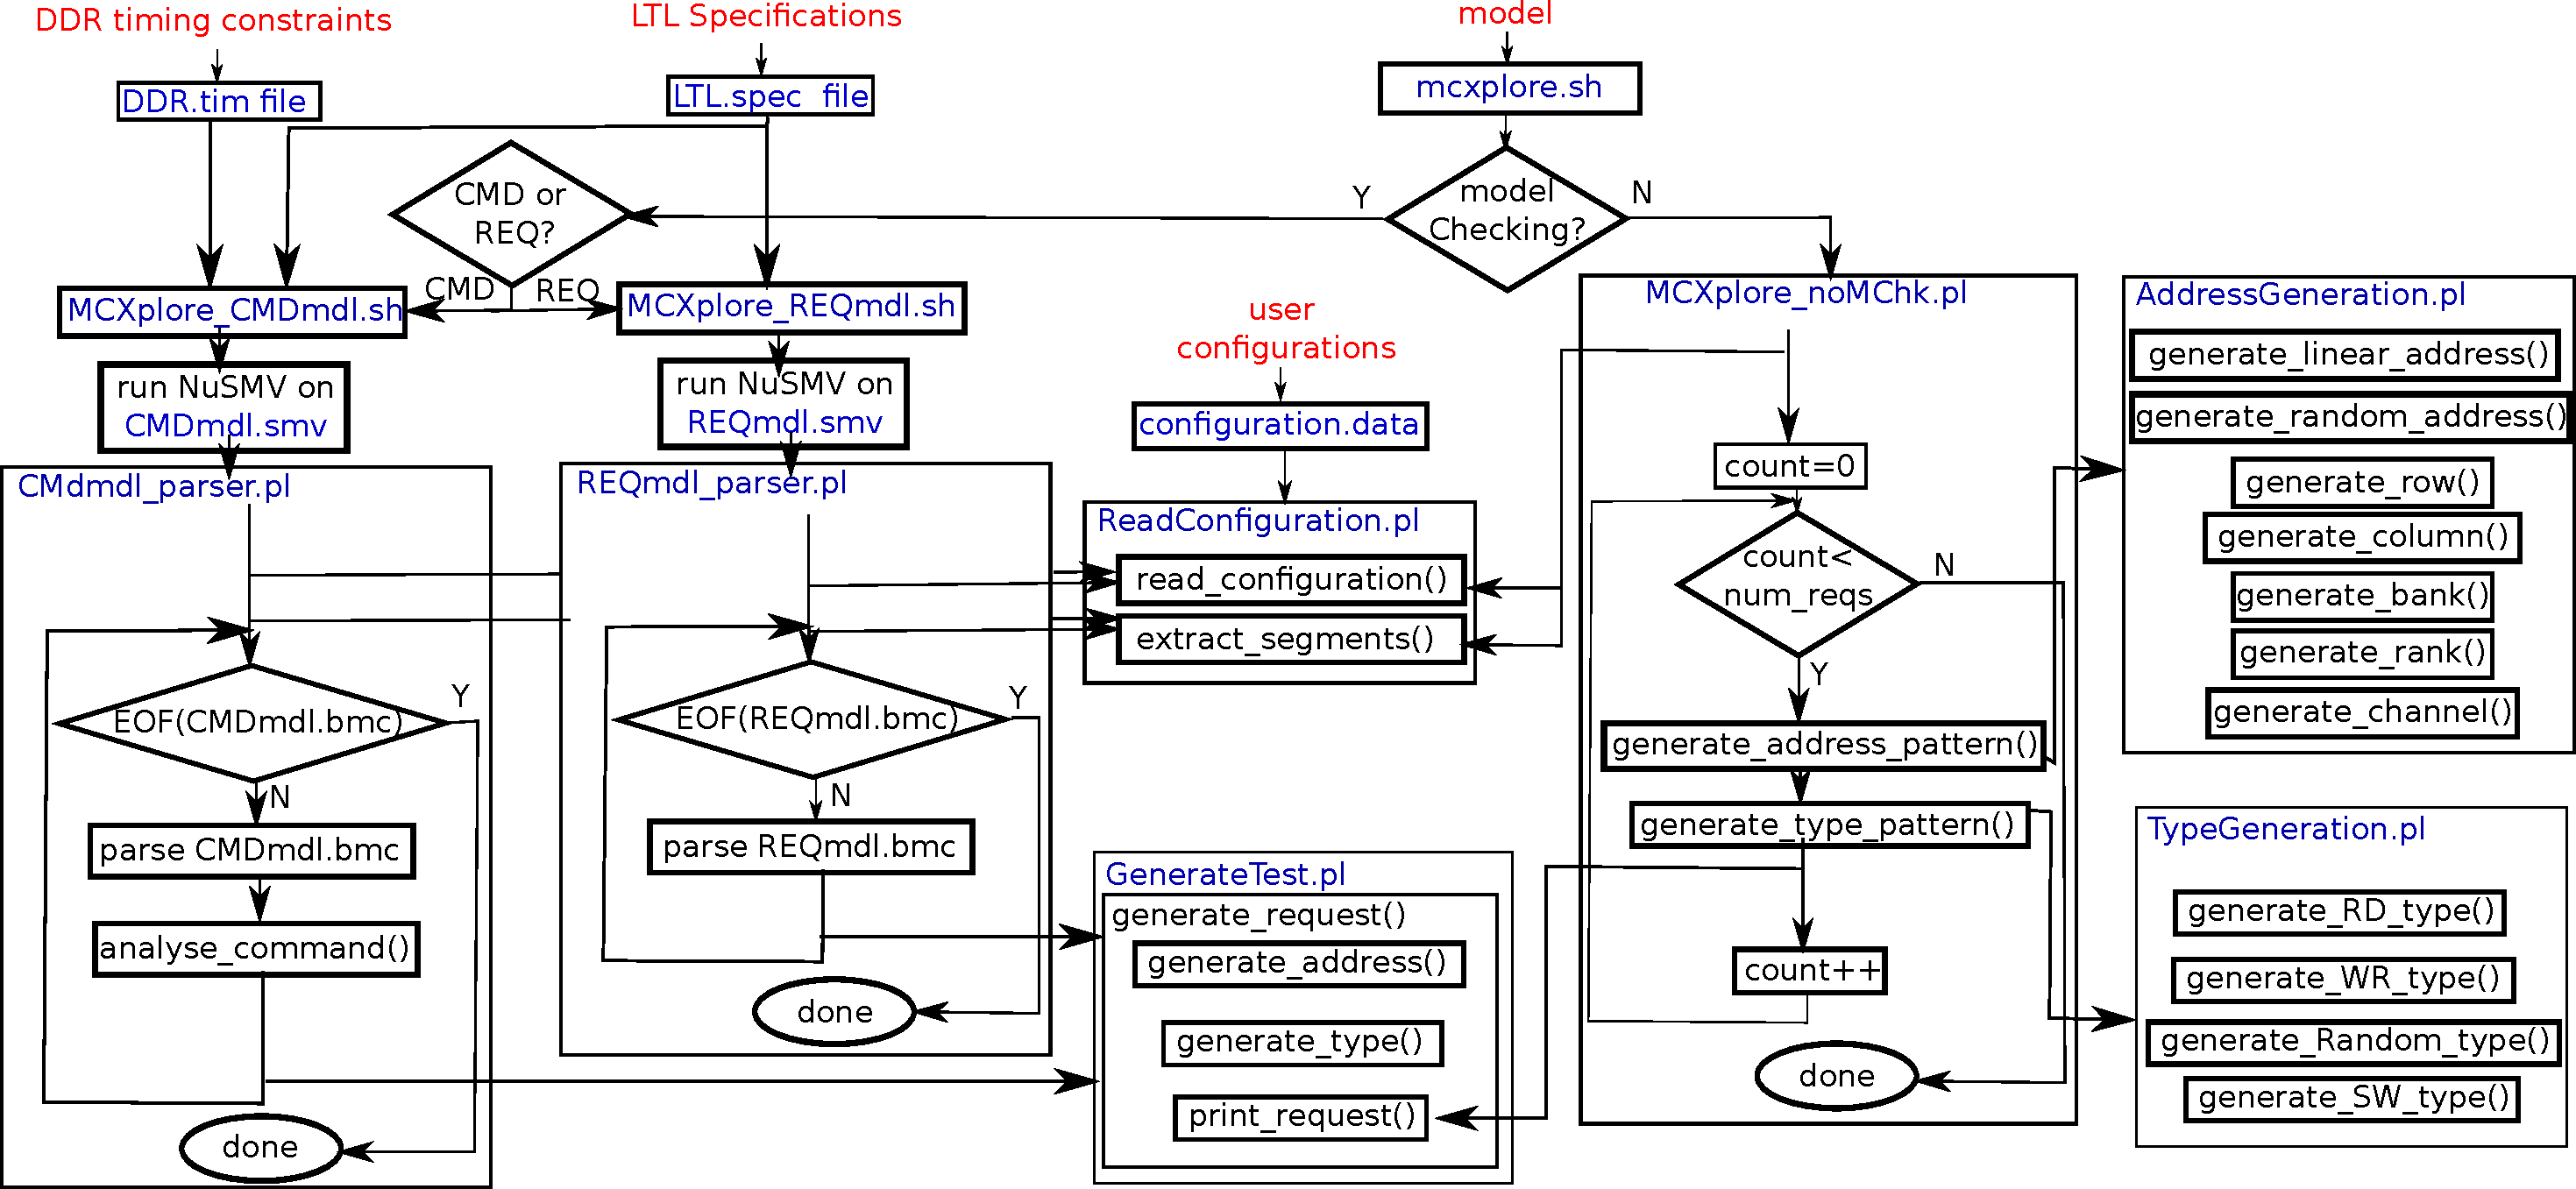
\includegraphics[scale=0.35]{MCXplore_flow.pdf}
\end{center}
\caption{MCXplore tool flow.~\label{fig:flow}}
\end{figure*} 


\section{Directory Structure} 
The top-level source directory of \textit{MCXplore} contains several directories. The list of those directories is the following: 

\begin{tabular}{|c|p{13.5cm}|}
\hline
/Docs & contains this documentation\\
/Mappings & contains address mapping schemes (\textbf{*.map} files) \\

/Models & contains the command interaction and request interrelation models\\ 

/NuSMV & should contain the NuSMV model checker tool\\ 

/LTLspec & contains the LTL specification files for the request and command models (\textbf{*.spec} files)\\

/DDrTimings & contains values of the DDR timing constraints, which are used by the command model (\textbf{*.tim} files)\\
/results & default directory for output test files\\

/TestSuites & contains test suites and regression tests that can be used to validate and evaluate most functionalities of modern memory controllers\\

/scripts & contains useful automation scripts to sweep configuration parameters\\
\hline
\end{tabular}

\section{Temporal Logic Specifications}\label{sec:TL}

NuSMV model checker allows for specifications expressed in Linear Temporal Logic (LTL). 
Typical LTL operations we use in \textit{MCXplore} are: \\

\begin{tabular}{|l|l|}
\hline
\textbf{F p} & Condition p holds in one of the future time instants\\

\textbf{G p} & Condition p holds in all of the future time instants\\

\textbf{p U q} & ondition p holds until a state is reached where condition q holds\\

\textbf{X p} & condition p is true in the next state\\
\hline
\end{tabular}\\

To help the user in properly setting the specifications, we accompany \textit{MCXplore} with a wide set of specifications for both the command interaction and the request interrelation models. 
Below are some examples of these specifications and their explanation. 
It is worth noting that all properties are negated such that the model checker produces the path, where this property holds.\\ 

\subsection{LTL specification examples for the request interrelation model}
\begin{enumerate}[leftmargin=*]
\item A test with $40\%$ bank interleaving and $20\%$ row locality:
\begin{lstlisting}[language=bash]
LTLSPEC G !(total_hit=2 & total_bank_interleave=4 & total_requests=10)
\end{lstlisting} 

\item A test with $34$ requests, all of them targeting same bank. 
Requests $1$ to $17$ target the same row, say $RW_1$. 
Requests $18$ to $34$ target the same row, say $RW_2$, which is different from $RW_1$, $RW_1 \neq RW_2$. 
This test can be used to test the adaptive page policy and First-Ready First-Come-First-Serve (FR-FCFS) arbitration with threshold as we illustrate in the DATE paper. 

\begin{lstlisting}[language=bash]
LTLSPEC G (consecutive_hit=16  -> ! F (total_bank_interleave=0 & total_
           requests=34 & consecutive_hit=16 & total_hit=32))
\end{lstlisting} 
\end{enumerate} 


\subsection{LTL specification examples for the command interaction model} 

The command interaction model is specifically useful for validating the correctness of the timing constraints and verifying that no timing violations occur due to any miss match between the memory controller and the DRAM. 
We refer the user to our DATE paper for more details about the command interaction model.

\begin{enumerate}[leftmargin=*]
\item Testing the Read-To-Precharge ($tRTP$) constraint. 
the intuition behind this specification is to make sure that the test sequence highlights the effect for $tRTP$ on the memory utilization. 
To assure this, the number of read commands has to be larger enough to subsumes the effect of the $tRAS$ constraint between the ACT command and the corresponding PRE command. 
The specification also ensures that all requests target the same bank by asserting that the number of read commands to a different bank or rank is zero. 
\begin{lstlisting}[language=bash]
G ! (((value_READ_TO_PRE_DELAY * num_READ_TO_PRE_DELAY + num_tCCD *
 value_tCCD + value_tRCD) > (value_tRAS)) & (num_READ_TO_PRE_DELAY > 0)
  & (num_Rx_d=0) & (num_Rd_s=0))
\end{lstlisting} 

\item Testing the CAS-to-CAS ($tCCD$) constraint. 
This specification creates requests targeting same bank and row. Hence, all requests except the first one will consist of a read command only. 
Each read command is separated by $tCCD$ cycles from the previous one. 


\begin{lstlisting}[language=bash]
G ! ((num_requests=50) & (num_tCCD=49) & ((num_tRL=1)|(num_tWL=1)) &
(num_tBUS=1) & (num_Rx_d=0))
\end{lstlisting} 
\end{enumerate} 

\section{Complete Examples}
\subsection{Request Model Example}
Consider the test with $40\%$ bank interleaving and $20\%$ row locality, with the following LTL specification:
\begin{lstlisting}[language=bash]
LTLSPEC G !(total_hit=2 & total_bank_interleave=4 & total_requests=10)
\end{lstlisting} 
running the \textit{MCxplore} flow for this test invokes the NuSMV model checker, which produces an intermediate file called \textbf{\textit{REQmdl.bmc}}. 
The contents of the  \textbf{\textit{REQmdl.bmc}} are shown below. 
\begin{lstlisting}[language=bash]
*** This is NuSMV 2.5.4 (compiled on Fri Oct 28 13:48:41 UTC 2011)
*** Enabled addons are: compass 
*** For more information on NuSMV see <http://nusmv.fbk.eu>
*** or email to <nusmv-users@list.fbk.eu>.
*** Please report bugs to <nusmv-users@fbk.eu>

*** Copyright (c) 2010, Fondazione Bruno Kessler

*** This version of NuSMV is linked to the CUDD library version 2.4.1
*** Copyright (c) 1995-2004, Regents of the University of Colorado

*** This version of NuSMV is linked to the MiniSat SAT solver. 
*** See http://www.cs.chalmers.se/Cs/Research/FormalMethods/MiniSat
*** Copyright (c) 2003-2005, Niklas Een, Niklas Sorensson 

WARNING *** This version of NuSMV is linked to the zchaff SAT         ***
WARNING *** solver (see http://www.princeton.edu/~chaff/zchaff.html). ***
WARNING *** Zchaff is used in Bounded Model Checking when the         ***
WARNING *** system variable "sat_solver" is set to "zchaff".          ***
WARNING *** Notice that zchaff is for non-commercial purposes only.   ***
WARNING *** NO COMMERCIAL USE OF ZCHAFF IS ALLOWED WITHOUT WRITTEN    ***
WARNING *** PERMISSION FROM PRINCETON UNIVERSITY.                     ***
WARNING *** Please contact Sharad Malik (malik@ee.princeton.edu)      ***
WARNING *** for details.                                              ***

WARNING: single-value variable 'max' has been stored as a constant
-- no counterexample found with bound 0
-- no counterexample found with bound 1
-- no counterexample found with bound 2
-- no counterexample found with bound 3
-- no counterexample found with bound 4
-- no counterexample found with bound 5
-- no counterexample found with bound 6
-- no counterexample found with bound 7
-- no counterexample found with bound 8
-- specification  G !((total_hit = 2 & total_bank_interleave = 4) &
-- total_requests = 10)    is false
-- as demonstrated by the following execution sequence
Trace Description: BMC Counterexample 
Trace Type: Counterexample 
-> State: 1.1 <-
  total_requests = 1
  row = same
  bank = same
  rank = same
  channel = same
  column = same
  consecutive_hit = 0
  consecutive_conflict = 0
  consecutive_bank_interleave = 0
  consecutive_same_bank = 0
  consecutive_rank_interleave = 0
  consecutive_same_rank = 0
  consecutive_channel_interleave = 0
  consecutive_same_channel = 0
  consecutive_column_interleave = 0
  consecutive_same_column = 0
  total_hit = 0
  total_bank_interleave = 0
  total_rank_interleave = 0
  total_channel_interleave = 0
  total_column_interleave = 0
  bool_same_row = FALSE
  bool_same_bank = TRUE
  bool_same_rank = FALSE
  bool_same_channel = TRUE
  bool_same_column = TRUE
  max = 10000
-> State: 1.2 <-
  total_requests = 2
  row = diff
  rank = diff
  consecutive_same_bank = 1
  consecutive_rank_interleave = 1
  consecutive_same_channel = 1
  consecutive_same_column = 1
  total_rank_interleave = 1
-> State: 1.3 <-
  total_requests = 3
  consecutive_same_bank = 2
  consecutive_rank_interleave = 2
  consecutive_same_channel = 2
  consecutive_same_column = 2
  total_rank_interleave = 2
-> State: 1.4 <-
  total_requests = 4
  consecutive_same_bank = 3
  consecutive_rank_interleave = 3
  consecutive_same_channel = 3
  consecutive_same_column = 3
  total_rank_interleave = 3
  bool_same_bank = FALSE
-> State: 1.5 <-
  total_requests = 5
  bank = diff
  consecutive_bank_interleave = 1
  consecutive_same_bank = 0
  consecutive_rank_interleave = 4
  consecutive_same_channel = 4
  consecutive_same_column = 4
  total_bank_interleave = 1
  total_rank_interleave = 4
  bool_same_rank = TRUE
-> State: 1.6 <-
  total_requests = 6
  rank = same
  consecutive_bank_interleave = 2
  consecutive_rank_interleave = 0
  consecutive_same_rank = 1
  consecutive_same_channel = 5
  consecutive_same_column = 5
  total_bank_interleave = 2
-> State: 1.7 <-
  total_requests = 7
  consecutive_bank_interleave = 3
  consecutive_same_rank = 2
  consecutive_same_channel = 6
  consecutive_same_column = 6
  total_bank_interleave = 3
  bool_same_rank = FALSE
  bool_same_channel = FALSE
  bool_same_column = FALSE
-> State: 1.8 <-
  total_requests = 8
  rank = diff
  channel = diff
  column = diff
  consecutive_bank_interleave = 4
  consecutive_rank_interleave = 1
  consecutive_same_rank = 0
  consecutive_channel_interleave = 1
  consecutive_same_channel = 0
  consecutive_column_interleave = 1
  consecutive_same_column = 0
  total_bank_interleave = 4
  total_rank_interleave = 5
  total_channel_interleave = 1
  total_column_interleave = 1
  bool_same_row = TRUE
  bool_same_bank = TRUE
  bool_same_rank = TRUE
  bool_same_channel = TRUE
-> State: 1.9 <-
  total_requests = 9
  row = same
  bank = same
  rank = same
  channel = same
  consecutive_hit = 1
  consecutive_bank_interleave = 0
  consecutive_same_bank = 1
  consecutive_rank_interleave = 0
  consecutive_same_rank = 1
  consecutive_channel_interleave = 0
  consecutive_same_channel = 1
  consecutive_column_interleave = 2
  total_hit = 1
  total_column_interleave = 2
  bool_same_column = TRUE
-> State: 1.10 <-
  total_requests = 10
  column = same
  consecutive_hit = 2
  consecutive_same_bank = 2
  consecutive_same_rank = 2
  consecutive_same_channel = 2
  consecutive_column_interleave = 0
  consecutive_same_column = 1
  total_hit = 2
  bool_same_row = FALSE
  bool_same_bank = FALSE
  bool_same_rank = FALSE
  bool_same_channel = FALSE
  bool_same_column = FALSE
\end{lstlisting}
This specific \textbf{\textit{REQmdl.bmc}} output illustrates that the bounded model checker runs for $10$ states ($0$ to $9$) until it reaches to a counter-example. 
This is clearly because we set the number of requests in the test to be $10$. 
Each state represents a unique request. 
The variables that maintain the same value as the previous state are not shown. 
For each address segment (row, column, ... etc.), it is either the "\textit{same}" or "\textit{diff}" compared to the previous request. 
all other variables in each state are counters to keep track of the address pattern. 
Afterwards, \textbf{\textit{REQmdl\_parser.pl}} parses this file and produces the required output test file as we show below. 
\begin{lstlisting}[language=bash]
0x00000000	R
0x00082000	R
0x00104000	R
0x00186000	R
0x00218000	R
0x002a8000	R
0x00338000	R
0x803ca040	R
0x803ca080	R
0x803ca080	R
\end{lstlisting} 

\subsection{Command Model Example}
Consider the test required to validate the $tRTP$ timing constraint, with the following LTL specification.
\begin{lstlisting}[language=bash]
G ! (((value_READ_TO_PRE_DELAY * num_READ_TO_PRE_DELAY + num_tCCD *
 value_tCCD + value_tRCD) > (value_tRAS)) & (num_READ_TO_PRE_DELAY > 0)
  & (num_Rx_d=0) & (num_Rd_s=0))
\end{lstlisting}
running the \textit{MCxplore} flow for this test invokes the NuSMV model checker, which produces an intermediate file called \textbf{\textit{CMDmdl.bmc}}. 
The contents of the  \textbf{\textit{CMDmdl.bmc}} are shown below.

\begin{lstlisting}[language=bash]
*** This is NuSMV 2.5.4 (compiled on Fri Oct 28 13:48:41 UTC 2011)
*** Enabled addons are: compass 
*** For more information on NuSMV see <http://nusmv.fbk.eu>
*** or email to <nusmv-users@list.fbk.eu>.
*** Please report bugs to <nusmv-users@fbk.eu>

*** Copyright (c) 2010, Fondazione Bruno Kessler

*** This version of NuSMV is linked to the CUDD library version 2.4.1
*** Copyright (c) 1995-2004, Regents of the University of Colorado

*** This version of NuSMV is linked to the MiniSat SAT solver. 
*** See http://www.cs.chalmers.se/Cs/Research/FormalMethods/MiniSat
*** Copyright (c) 2003-2005, Niklas Een, Niklas Sorensson 

WARNING *** This version of NuSMV is linked to the zchaff SAT         ***
WARNING *** solver (see http://www.princeton.edu/~chaff/zchaff.html). ***
WARNING *** Zchaff is used in Bounded Model Checking when the         ***
WARNING *** system variable "sat_solver" is set to "zchaff".          ***
WARNING *** Notice that zchaff is for non-commercial purposes only.   ***
WARNING *** NO COMMERCIAL USE OF ZCHAFF IS ALLOWED WITHOUT WRITTEN    ***
WARNING *** PERMISSION FROM PRINCETON UNIVERSITY.                     ***
WARNING *** Please contact Sharad Malik (malik@ee.princeton.edu)      ***
WARNING *** for details.                                              ***

WARNING: single-value variable 'value_tRP' has been stored as a constant
WARNING: single-value variable 'value_tCCD' has been stored as a constant
WARNING: single-value variable 'value_tRAS' has been stored as a constant
WARNING: single-value variable 'value_tRC' has been stored as a constant
WARNING: single-value variable 'value_tRCD' has been stored as a constant
WARNING: single-value variable 'value_tRRD' has been stored as a constant
WARNING: single-value variable 'value_tFAW' has been stored as a constant
WARNING: single-value variable 'value_tRL' has been stored as a constant
WARNING: single-value variable 'value_tWL' has been stored as a constant
WARNING: single-value variable 'value_tRTP' has been stored as a constant
WARNING: single-value variable 'value_tWR' has been stored as a constant
WARNING: single-value variable 'value_tWTR' has been stored as a constant
WARNING: single-value variable 'value_tRTRS' has been stored as a constant
WARNING: single-value variable 'value_tBUS' has been stored as a constant
WARNING: single-value variable 'value_READ_TO_WRITE_DELAY' 
has been stored as a constant
WARNING: single-value variable 'value_RANK_TO_RANK_DELAY' 
has been stored as a constant
WARNING: single-value variable 'value_READ_TO_PRE_DELAY' 
has been stored as a constant
WARNING: single-value variable 'value_WRITE_TO_READ_DELAY_B'
 has been stored as a constant
WARNING: single-value variable 'value_WRITE_TO_READ_DELAY_R'
 has been stored as a constant
WARNING: single-value variable 'value_WRITE_TO_PRE_DELAY'
 has been stored as a constant
WARNING: single-value variable 'max' has been stored as a constant
Warning: cannot assign value 10001 to variable num_Rx_d
Warning: cannot assign value 10001 to variable num_Rd_s
-- no counterexample found with bound 0
-- no counterexample found with bound 1
-- no counterexample found with bound 2
-- no counterexample found with bound 3
-- no counterexample found with bound 4
-- specification  G !((((value_READ_TO_PRE_DELAY * num_READ_TO_PRE_DELAY +
-- num_tCCD * value_tCCD) + value_tRCD > value_tRAS &
--  num_READ_TO_PRE_DELAY > 0) & num_Rx_d = 0) & num_Rd_s = 0)
--   is false
-- as demonstrated by the following execution sequence
Trace Description: BMC Counterexample 
Trace Type: Counterexample 
-> State: 1.1 <-
  num_requests = 0
  num_tRP = 0
  num_tCCD = 0
  num_tRAS = 0
  num_tRC = 0
  num_tRCD = 0
  num_tRRD = 0
  num_tFAW = 0
  num_tRL = 0
  num_tWL = 0
  num_tRTP = 0
  num_tWR = 0
  num_tWTR = 0
  num_tRTRS = 0
  num_tBUS = 0
  num_Rd_s = 0
  num_Rx_d = 0
  num_READ_TO_WRITE_DELAY = 0
  num_RANK_TO_RANK_DELAY = 0
  num_READ_TO_PRE_DELAY = 0
  num_WRITE_TO_READ_DELAY_B = 0
  num_WRITE_TO_READ_DELAY_R = 0
  num_WRITE_TO_PRE_DELAY = 0
  activated_banks = 0
  command = As_s
  constraint = RANK_TO_RANK_DELAY
  value_tRP = 10
  value_tCCD = 4
  value_tRAS = 24
  value_tRC = 34
  value_tRCD = 10
  value_tRRD = 4
  value_tFAW = 20
  value_tRL = 10
  value_tWL = 9
  value_tRTP = 5
  value_tWR = 10
  value_tWTR = 5
  value_tRTRS = 1
  value_tBUS = 4
  value_READ_TO_WRITE_DELAY = 6
  value_RANK_TO_RANK_DELAY = 5
  value_READ_TO_PRE_DELAY = 5
  value_WRITE_TO_READ_DELAY_B = 18
  value_WRITE_TO_READ_DELAY_R = 4
  value_WRITE_TO_PRE_DELAY = 23
  max = 10000
-> State: 1.2 <-
  num_requests = 1
  num_tRCD = 1
  command = Rs_s
  constraint = tRCD
-> State: 1.3 <-
  num_requests = 2
  num_tCCD = 1
  constraint = tCCD
-> State: 1.4 <-
  num_requests = 3
  num_tCCD = 2
-> State: 1.5 <-
  num_requests = 4
  num_tCCD = 3
-> State: 1.6 <-
  num_READ_TO_PRE_DELAY = 1
  command = P
  constraint = READ_TO_PRE_DELAY
\end{lstlisting} 

Afterwards, \textbf{\textit{CMDmdl\_parser.pl}} parses this file and produces the required output test file as we show below. 
\begin{lstlisting}[language=bash]
0x00000000	R
0x00000040	R
0x00000080	R
0x000000c0	R
\end{lstlisting} 
\externaldocument{configuration_tbl}
\section{Test Suites} 
We accompany \textit{MCxplore} with sets of regression tests to validate and evaluate most of the modern memory controller properties. 
Namely, we provide three test suites based on the model we use to generate this test suite. All test suites reside in the TestSuites subdirectory. 
Table~\ref{tb:suites} tabulates these test suites.

\begin{table}[h]
\caption{Test Suites\label{tb:suites}}
\begin{tabular}{|c|c|p{11cm}|}
\hline
Suite & Model used & Description\\
\hline
regressionSuite & noMChk & this suite includes tests that cover all combinations of the configuration parameters in Table~\ref{tb:config_noMChk}\\
\hline 

PoliciesSuite & REQmdl & this suite includes tests that test most commonly used policies of commodity memory controllers such as page policies, address mapping and arbitration schemes.\\
\hline

TimingSuites & CMDmdl & this suite includes tests to detect any timing violations in most timing constraints\\
\hline
\end{tabular}
\end{table}


\section{Citation} 
If your use of \textit{MCXplore} contributes to a published paper, please cite our  DATE research paper. 
The paper can be downloaded from here:

\url{https://ece.uwaterloo.ca/~m49hassa/publications/MCXplore_DATE16.pdf} 

The bibtex citation is: 

\begin{lstlisting}
@inproceedings{MCxplore,
  title={MCXplore: An Automated Framework for Validating Memory Controller 
  Designs},
  author={Hassan, Mohamed and Patel, Hiren},
  booktitle={ IEEE Conference on Design, Automation and Test in Europe
   (DATE) },
  year={2016}

}
\end{lstlisting}
\end{document}

